% ------------------------------------------------------------------------------
% TYPO3 CMS 8.4 - What's New - Chapter "Backend User Interface" (Italian Version)
%
% @author	Michael Schams <schams.net>
% @license	Creative Commons BY-NC-SA 3.0
% @link		http://typo3.org/download/release-notes/whats-new/
% @language	English
% ------------------------------------------------------------------------------
% LTXE-CHAPTER-UID:		07b25346-95b1df21-a6ebe09a-49f53f41
% LTXE-CHAPTER-NAME:	Backend User Interface
% ------------------------------------------------------------------------------

\section{Interfaccia utente Backend}
\begin{frame}[fragile]
	\frametitle{Interfaccia utente Backend}

	\begin{center}\huge{Capitolo 1:}\end{center}
	\begin{center}\huge{\color{typo3darkgrey}\textbf{Interfaccia utente Backend}}\end{center}

\end{frame}

% ------------------------------------------------------------------------------
% LTXE-SLIDE-START
% LTXE-SLIDE-UID:		d7aa5777-d02e5a2f-fc912afd-98c8d753
% LTXE-SLIDE-ORIGIN:	75977160-b74e3317-0f697728-71b501d1 English
% LTXE-SLIDE-TITLE:		Mobile Responsive TYPO3 Backend
% ------------------------------------------------------------------------------

\begin{frame}[fragile]
	\frametitle{Interfaccia utente Backend}
	\framesubtitle{Backend TYPO3 responsivo}

	Ora il backend di TYPO3 Backend è completamente responsivo per mobile.

	\begin{figure}
		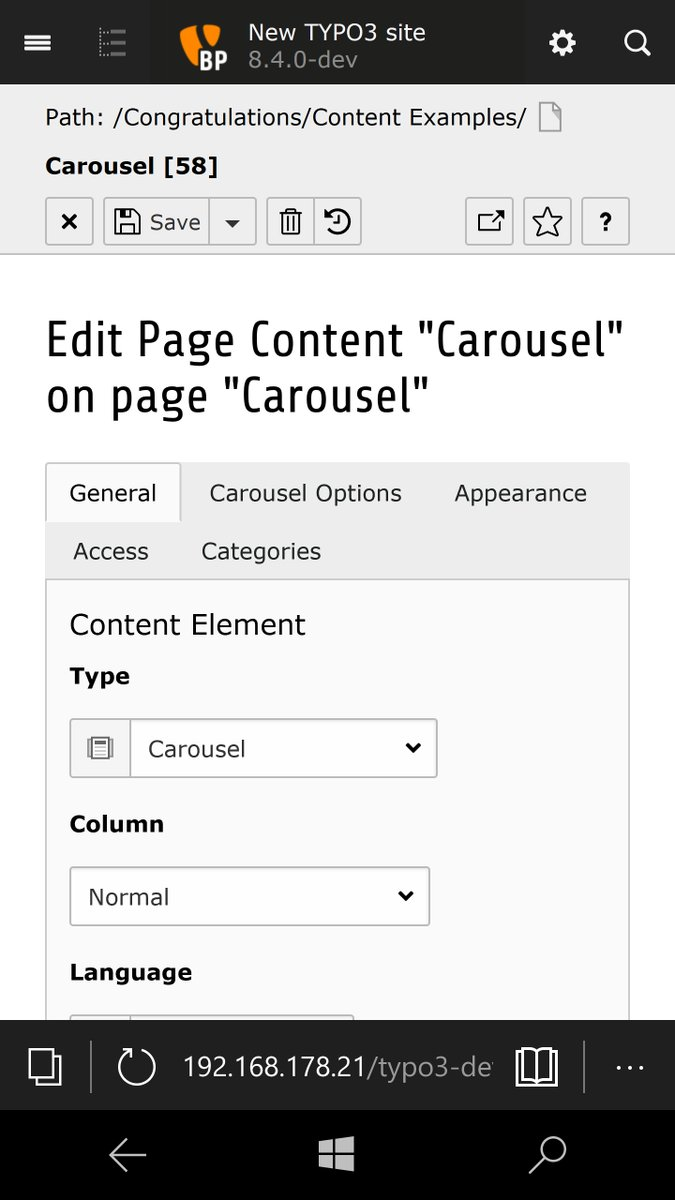
\includegraphics[width=0.25\linewidth]{BackendUserInterface/mobile-responsive-backend.jpg}
	\end{figure}

\end{frame}

% ------------------------------------------------------------------------------
% LTXE-SLIDE-START
% LTXE-SLIDE-UID:		30d05641-cfb09a80-032704ff-00342a38
% LTXE-SLIDE-ORIGIN:	f6668b2d-8932a470-5b9c024c-e4e9f53a English
% LTXE-SLIDE-TITLE:		Install Tool: Upgrade Analysis
% ------------------------------------------------------------------------------

\begin{frame}[fragile]
	\frametitle{Interfaccia utente Backend}
	\framesubtitle{Install Tool: analisi upgrade}

% The install tool, which is also a heavily used feature during updates between
% TYPO3 versions, has received some more beauty, basically finding all documented
% changes with a cool filter to show what is relevant for an integrator,
% extension author or site owner. Although this is already pretty cool, stay
% tuned for even better features to make migrations even easier between TYPO3
% versions!
% The migration and deprecation of existing options and switching within the TCA
% definitions we have in place since TYPO3 v7, is also visible in the Install Tool
% now.

	L'upgrade di versione TYPO3 risulta più facile con il nuovo tool di \textbf{Upgrade Analysis}
	nell'Install Tool (cerca/filtra tutte le modifiche documentate tra le due versioni).

	\begin{figure}
		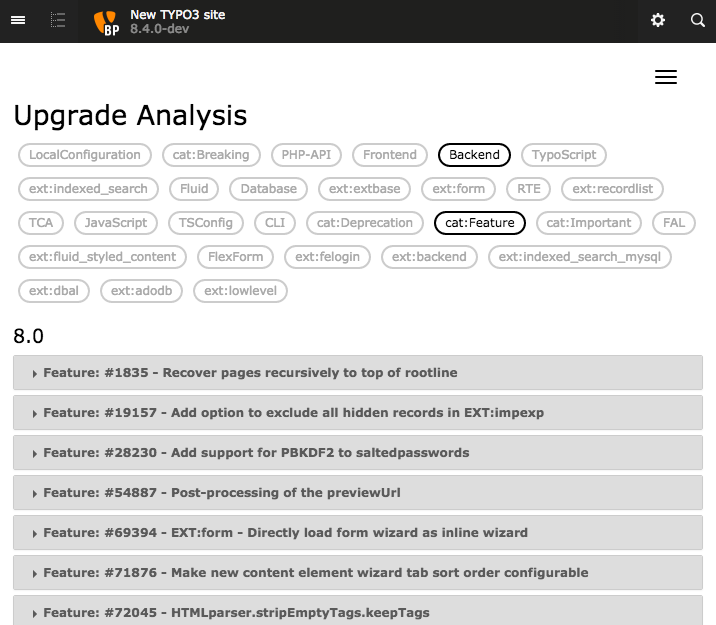
\includegraphics[width=0.45\linewidth]{BackendUserInterface/install-tool-upgrade-analysis.png}
	\end{figure}

\end{frame}

% ------------------------------------------------------------------------------
% LTXE-SLIDE-START
% LTXE-SLIDE-UID:		81eca23f-e99a165b-f793ee8f-1bac000d
% LTXE-SLIDE-ORIGIN:	9702aaf4-f02bbc35-67902b2e-42855506 English
% LTXE-SLIDE-TITLE:		Install Tool: Upgrade Analysis
% LTXE-SLIDE-REFERENCE:	#78222: Dump Class Loading Information UI in Install Tool
% ------------------------------------------------------------------------------

\begin{frame}[fragile]
	\frametitle{Interfaccia utente Backend}
	\framesubtitle{Install Tool: Dump Autoload Information}

	Per rigenerare le informazioni caricate automaticamente dalle classi, è stata aggiunta una nuova azione
	nell'Install Tool per fare il dump di esse.

	\begin{figure}
		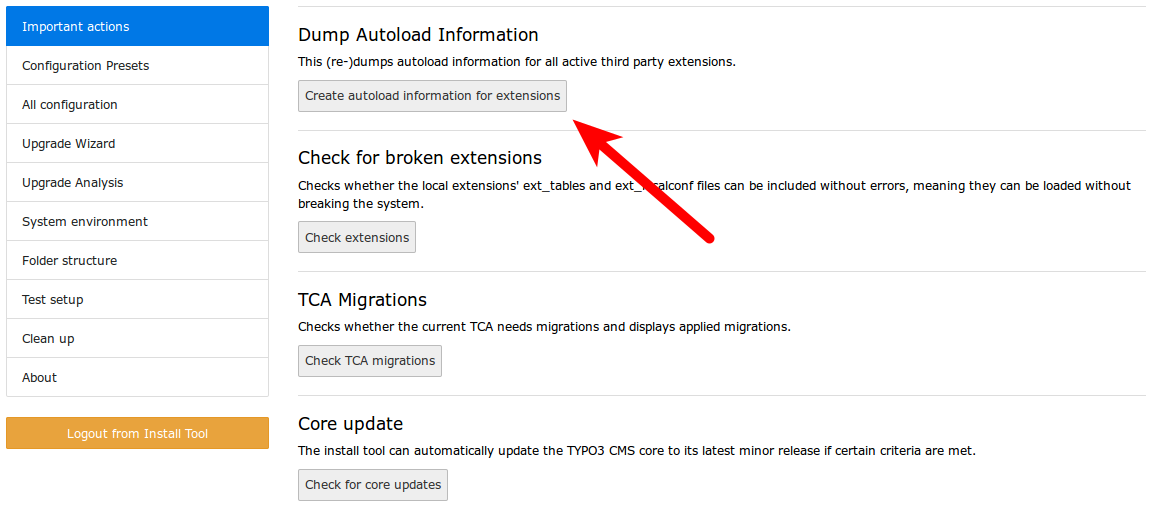
\includegraphics[width=0.8\linewidth]{BackendUserInterface/78222.png}
	\end{figure}

\end{frame}

% ------------------------------------------------------------------------------
% LTXE-SLIDE-START
% LTXE-SLIDE-UID:		bca91288-69367b9c-3a509609-9d28420d
% LTXE-SLIDE-ORIGIN:	5a194e82-8eac7f1b-ef2730da-61d781b2 English
% LTXE-SLIDE-TITLE:		Install Tool: TCA Migration Messages
% LTXE-SLIDE-REFERENCE:	#77799: Display TCA migration messages in Install Tool
% ------------------------------------------------------------------------------

\begin{frame}[fragile]
	\frametitle{Interfaccia utente Backend}
	\framesubtitle{Install Tool: TCA Migration Messages}

	I messaggi di migrazione del TCA possono essere selezionati/elencati nell'Install Tool.

	\begin{figure}
		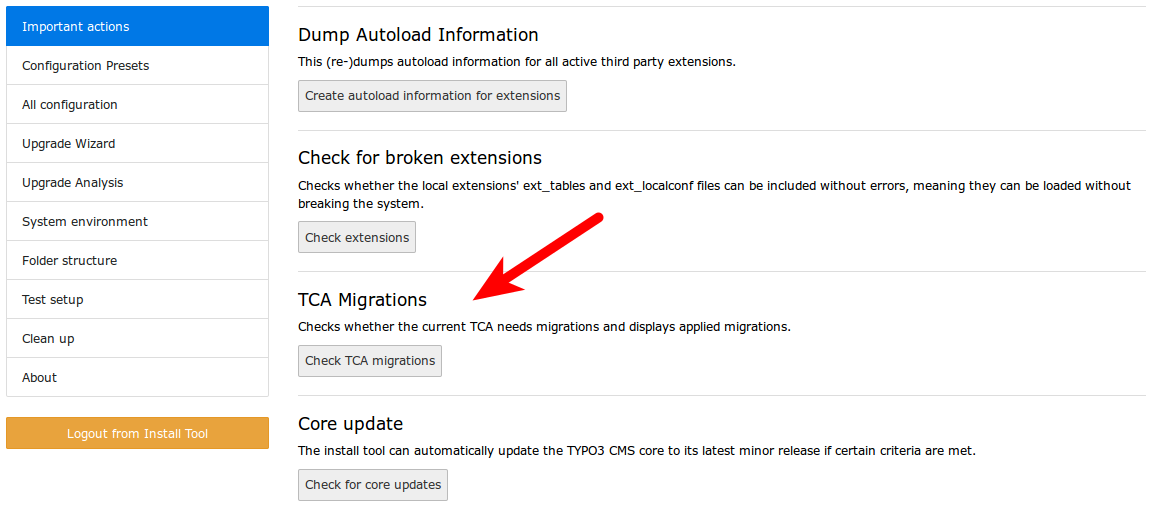
\includegraphics[width=0.8\linewidth]{BackendUserInterface/77799.png}
	\end{figure}

\end{frame}

% ------------------------------------------------------------------------------
% LTXE-SLIDE-START
% LTXE-SLIDE-UID:		c48e0d32-34edac35-90cc8276-264b42be
% LTXE-SLIDE-ORIGIN:	1e11eae3-872938ec-9612c092-444c408a English
% LTXE-SLIDE-TITLE:		sys_language records are sortable now
% LTXE-SLIDE-REFERENCE:	#77652: Make sys_language records sortable
% ------------------------------------------------------------------------------

\begin{frame}[fragile]
	\frametitle{Interfaccia utente Backend}
	\framesubtitle{\texttt Record {sys\_language}}

	Per migliorare l'usabilità, ora è possibile ordinare i record \texttt{sys\_language}.

	\begin{figure}
		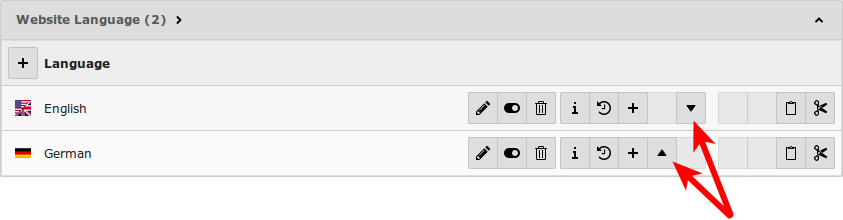
\includegraphics[width=0.8\linewidth]{BackendUserInterface/77652.png}
	\end{figure}

\end{frame}

% ------------------------------------------------------------------------------
% LTXE-SLIDE-START
% LTXE-SLIDE-UID:		ce586a08-02175441-59730c1e-cff8a287
% LTXE-SLIDE-ORIGIN:	a82823ff-94b9520f-5e6d6056-95f1a797 English
% LTXE-SLIDE-TITLE:		#77668: Hide table listing below group element
% ------------------------------------------------------------------------------

\begin{frame}[fragile]
	\frametitle{Interfaccia utente Backend}
	\framesubtitle{Table Listing Below Group Element}

	\begin{itemize}

		\item L'opzione di configurazione del TCA \texttt{disable\_controls} del tipo "group"
			ha la nuova impostazione \texttt{allowedTables}. Essa permette di nascondere i suggerimenti delle
			tabelle autorizzate ad essere referenziate nelle selezioni del campo.

	\end{itemize}

	\begin{figure}
		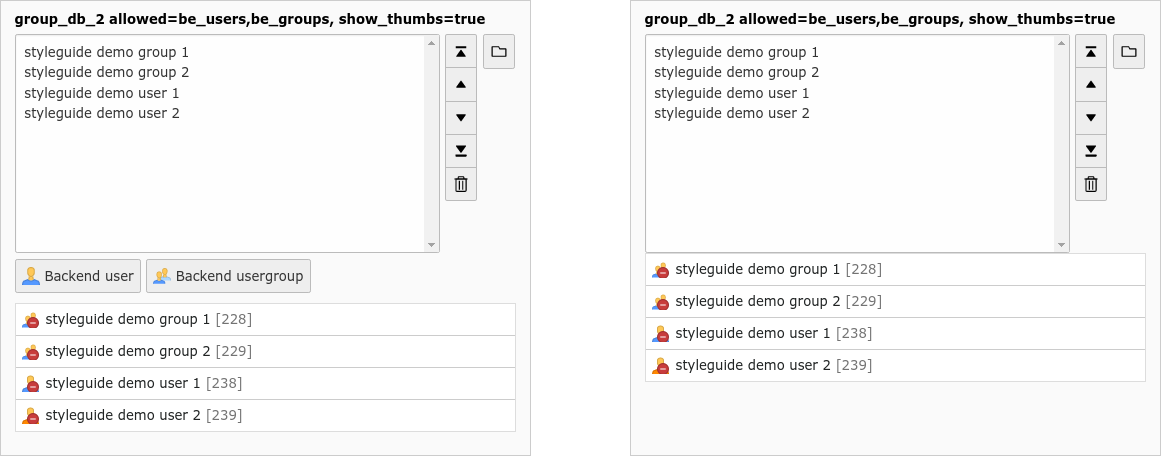
\includegraphics[width=0.85\linewidth]{BackendUserInterface/77668.png}
	\end{figure}

\end{frame}

% ------------------------------------------------------------------------------
